\section{Introduction}
\label{sec:intro}

In this paper, we study data on VirusTotal submitted from 2016/05/07 to 2016/09/06 (Figure~\ref{fig:subnum}). 
Our study is conducted from three aspects:



\begin{figure}[t!]
\begin{center}
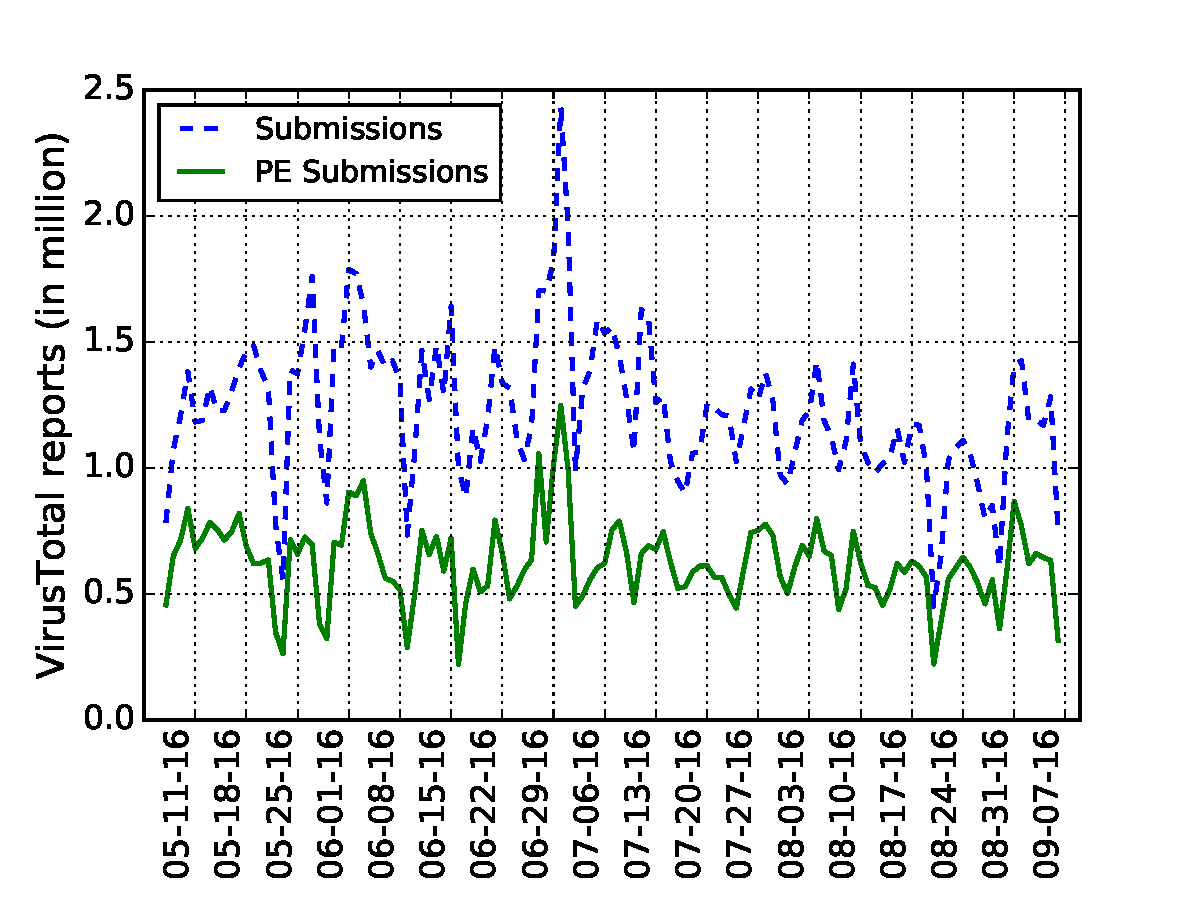
\includegraphics[width=2.5in]{figure/Submissions}
\mycaption{fig:subnum}{The number of files and PE files.}
{\footnotesize{(The number of suspicious files and the number of PE files submitted to VirusTotal from 05/07/2016 to 09/06/2016.)
}}
\end{center}
%\vspace{-0.25in}
\end{figure}


First, we study the correlation between submissions' metadata and their detection rates. 
For each submission, VirusTotal will apply more than one anti-virus engines to analyze it. 
Some engines will identify the submission as malware, while others will not. 
We use the percentage of engines identifying the malware to describe the likelihood of the malware getting detected. 
To study the correlation between submissions' metadata and their detection rates, 
we can understand and characterize which malwares are more likely to be detected.   

Second, we study influence among different antivirus vendors. 
One malware could be submitted to VirusTotal more than once. 
For each submission, VirusTotal will apply a bunch of anti-virus engines to analyze it.
We have observed that for some malwares, some anti-virus engines fail to detect them at the first time, while they catch up in later analysis. 
We assume that there is influence among different anti-virus vendors, 
and some anti-virus vendors will follow detection results from other vendors. 
We apply models from web social network area to characterize 
which vendors are more likely to be influenced by others, 
and predict whether detection results from some vendors may change in the future.  

Third, we build a malware detector and classifier based on ssdeep similarity. 
SSDeep is a fuzzy hash algorithm, which takes a file as input and generates a fuzzy hash string as information digest. 
The similarity between fuzzy hashes is an estimation of similarity between the two original files. 
Fuzzy hash for each submission is also calculated and provided by VirusTotal. 
We explore how to use similarity between SSDeep fuzzy hash as 
kernel function to conduct malware classification and malware detection. 